\chapter{Seminario 2: \textit{Computer Vision and Medical Imaging}}

Dal professore e ricercatore del Dipartimento di Matematica e informatica dell'Università di Cagliari, Andrea Loddo.

\section{Intelligenza Artificiale}
Come siamo arrivati a parlare di intelligenza artificiale al giorno d'oggi? L'intelligenza artificiale non è altro che un termine per trattare degli elementi che fanno capo al Machine Learning.
Non è sbagliato dire che \textbf{le fondamenta dell'AI sono radicate nel Machine Learning}.

\subsection{Machine Learning}
Non programmare esplicitamente la soluzione ad un problema, ma insegnare ad una macchina  delle regole partendo da un insieme di dati che rappresenta il problema. 

\subsection{Machine learning e Deep Learning}

Se il Deep Learning è alla base di molte delle soluzioni moderne, perché ha ancora senso parlare di Machine Learning?

\paragraph{Pertinenza del modello rispetto al task.} Nel machine learning, le procedure di learning sono più rapide, e operano su meno dati rispetto al DL. I modelli sono più facilmente interpretabili. In un mondo fatto da così tanti task e problemi differenti, \textit{non è opportuno parlare di modelli vecchi, ma piuttosto, di modelli adatti.} 

\paragraph{Il machine learning è il punto di partenza.} Non dobbiamo dimenticare che il Deep Learning nasce dal Machine Learning, e non può fare a meno dei suoi fondamenti.

\section{Caso studio 1: radiomica}
Per \textbf{radiomica} si intende l'\textbf{analisi delle immagini mediche} volta a ottenere, tramite opportuni metodi matematici e i calcolatori, \textbf{informazioni di tipo quantitativo} da queste \textbf{non rilevabili tramite la loro semplice osservazione visiva} da parte dell'operatore.
Le informazioni in questione dovranno essere \textbf{significative}, in quanto volte ad un supporto allo specialista, come nel caso delle diagnosi clinica.

\paragraph{Perché è rilevante?}
La radiomica permette di evitare esami molto invasivi, come le \textbf{biopsie}, alzando comunque il livello di accuratezza delle diagnosi. Il processo radiomico può essere integrato nel campo medico, al fine di migliorarlo. Dalle immagini è anche possibile ottenere rappresentazioni numeriche di ciò che il radiologo vede, o trovare pattern nascosti ma rilevanti.

\paragraph{Biomarcatori.}
Definiamo biomarcatore una caratteristica misurabile nell'organismo che fornisce informazioni oggettive sullo stato di salute. Gli output dei nostri modelli dovranno essere fortemente influenzate dai biomarcatori rilevati.

\subsection{Pipeline radiomica}

\paragraph{Acquisire le immagini.} Raggi-X, risonanze, ultrasuoni, etc. Queste possono venire da \textbf{sorgenti e macchinari differenti}. Questi useranno \textbf{protocolli} molto \textbf{differenti}. Bisogna essere anche molto attenti sul cosa si acquisisce, evitando di catturare informazioni non-necessarie o fuorvianti. Insomma, acquisire i dati è uno step molto delicato.

\paragraph{Processing dell'input.} Tra cui \textbf{resampling} e \textbf{quantizzazione}, per ridurre la risoluzione dell'informazione e dei livelli di grigio.

\paragraph{Segmentazione.} Da un'immagine che rappresenta un'oggetto, ridurre l'analisi ad una sola parte dell'immagine. Può essere effettuata manualmente, in maniera semi-automatica o del tutto automatica. In alternativa, si possono delineare dei bounding-box, applicando un algoritmo di \textbf{object detection}.

\paragraph{Estrazione delle features.} Un'immagine è una matrice di numeri. Cosa ce ne facciamo di questi numeri? Bisogna dare una forma sensata, e soprattutto \textbf{significativa} a questi numeri. Esistono vari modi di estrarre features. Tra questi: histogram based, texture based, shape based, transform based e deep features extraction.

\paragraph{Analisi delle features e dei campioni.} È importante analizzare i campioni, per diagnosticare circostanze di \textbf{oversampling} e \textbf{undersampling} sulle varie classi. Si possono anche applicare tecniche di \textbf{normalizzare} delle features o di \textbf{riduzione delle features}, per evitare la \textit{Curse of Dimensionality}\footnote{La \textit{Curse of Dimensionality} un fenomeno nel machine learning dove le prestazioni e l'efficacia degli algoritmi si deteriorano all'aumentare del numero di variabili (dimensioni) in un dataset, rendendo i dati sparsi e le relazioni difficili da trovare, aumentando esponenzialmente la complessità computazionale e il rischio di overfitting}. In particolar modo, il problema della riduzione delle features non è triviale in alcun modo: ogni tecnica ha infatti pro e contro. Creare features basate su quelle di partenza, crea nuovi dati. Estrarre un sottoinsieme di features, rischia di non rappresentare in maniera opportuno il dominio dei dati.

\paragraph{Costruzione e valutazione del modello.} Tramite approcci supervised o unsupervised, e valutare i vari modelli tramite i vari parametri e metriche che è possibile calcolare.

\subsection{Work 1: feature extraction }
Presentiamo alcune conclusioni sulle tecniche usate in alcuni lavori effettuati dal gruppo di ricerca nel campo della radiomica.

\paragraph{Si preferiscono informazioni mirate.} Le informazioni puntuali, relative alle zone di interesse, sono più comunicative rispetto alle features che rappresentano l'intera immagine. 

\paragraph{Interpretabilità nei modelli.} È difficile capire i motivi dietro agli output di alcuni modelli. Nel machine learning, tramite visualizzazioni come la \textbf{GradCam}, è possibile mappare in una heatmap le zone d'interesse principali del modello. Nel machine learning, per capire la rilevanza delle features, usiamo metodi come:

\begin{itemize}
	\item \textbf{SHAP} (SHapley Additive exPlanations): questa, permette di capire la rilevanza di ciascuna delle features, e i motivi per cui il modello ha preso determinate decisioni, andando oltre la black-box.
	
	\item \textbf{Metodo della correlazione}: se due features sono estremamente correlate, ne basta una per dare informazioni pertinenti.
\end{itemize} 

Questi due metodi si occupano quindi di analizzare rispettivamente la correlazione feature-label (desiderata), e la correlazione feature-feature (non desiderata). Queste metodologie permettono di effettuare scelte di feature reduction/selection opportune.

\subsection{Work 2: Dynamic Feature Selection (DFS)}
L'idea è quella di stabilire dinamicamente le features da considerare, in funzione dello stato del modello, del contesto o dell'input ricevuto. Un modello di input, permette di selezionare il peso di ognuna delle features in maniera opportuna. L'utilizzo di questa metodologia ha permesso di ottenere risultati strabilianti sul dataset MNIST, con un'accuracy in testing del 98\% con una sola feature. Le performance calano su dataset a risoluzione maggiore e a colori: nonostante ciò, rispetto allo stato dell'arte degli altri algoritmi dinamici, anche un risultato come 0.18 in evaluation è significativo.

\subsection{Work 3: Federated Feature Selection}
Questa tecnica di feature selection si basa su alcune intuizioni che nascono dal \textbf{federated learning}.

\paragraph{Federated Learning}
È una tecnica di machine learning decentralizzata che addestra modelli di IA collaborativi su dati distribuiti, mantenendo le informazioni sensibili sui dispositivi locali senza condividerle. È opportuno al campo medico, in quanto i dati di training non possono essere diffusi.

\paragraph{Federated Feature Selection}
In questo caso, si contribuisce al modello federato non più con i pesi (che rappresentano come le immagini una forma di informazione sensibile relativa ai pazienti, al contrario di quello che si potrebbe pensare), ma con la rilevanza delle features. Questo permette al modello federato di stabilire il modo con cui i client debbano effettuare la feature selection. I risultati del modello server, valgono per i modelli di tutti i client: considerati due client $A,B$, questi potrebbero usare dispositivi di acquisizione differenti e modelli molto differenti, ma a parità di tipologia di dati, le features significative sono le stesse.


\section{Caso studio 2: immagini di cellule del sangue nei vetrini}

Ho delle immagini ottenute da dei vetrini, su cui viene ossidato del sangue. Dai vetrini, tiro delle immagini al microscopio. L'immagine può comprendere tre sezioni d'interesse: globuli bianchi, globuli rossi e piastrine. Questo caso studio non è stato approfondito particolarmente a causa dei limiti di tempo, ma è stata offerta una analisi di alcune delle criticità principali, del task, e di alcune soluzioni.


\section{Machine Learning is not dead.}
Delle tecniche, che al giorno d'oggi sono considerate datate e fuorimercato, in realtà ci offrono le fondamenta per le tecniche ritenute moderne, e rimangono comunque viabili. Tutto dipende dal task che si sta affrontando, e da come i dati sono catturati e trattati.

\begin{figure}[tbph]
	\centering
	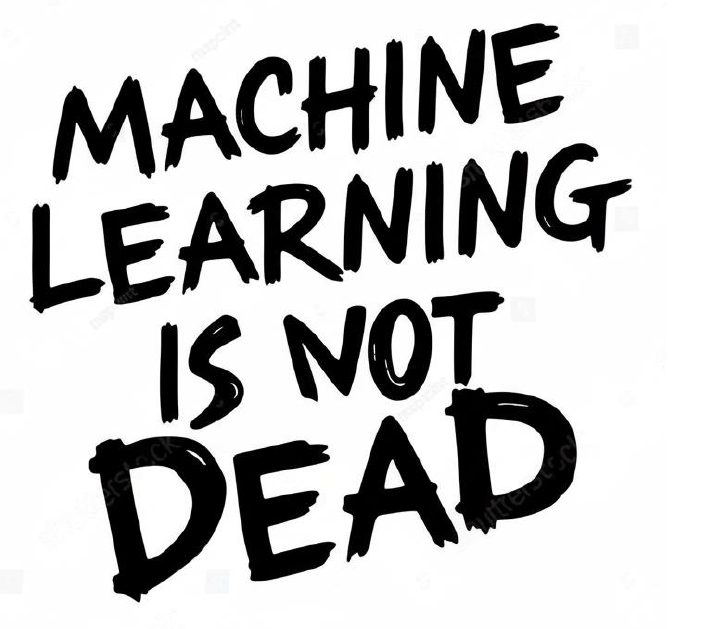
\includegraphics[width=0.5\linewidth]{./images/machine-learning-is-not-dead}
\end{figure}

